% Paste this block immediately after the Task subsection.
% It is a fragment only. Do not add \documentclass, \begin{document}, or \end{document}.

\newcommand{\mechplaceholderfig}[1]{%
  \fbox{\begin{minipage}[c][0.15\textheight][c]{0.80\textwidth}\centering\itshape #1\end{minipage}}}

% Works in both text and math mode, so this fragment does not require siunitx.
\newcommand{\mechSI}[2]{\ensuremath{#1\,\mathrm{#2}}}

\subsection{Mechanical Design and Modeling}\label{sec:mechanical_design}

The mechanical design presents the physical platform and the models that describe its motion and loading. It addresses the mechanical architecture, the CAD and digital twin pipeline, the kinematic and dynamic models of the manipulator, the collision representation, and the experimental identification of the joint and motor parameters. All kinematic and dynamic relations were verified symbolically and numerically against the implementation in \texttt{works/}.

\subsubsection{Mechanical System Overview}\label{sec:mech_overview}
The robot is a mobile manipulator built from four subsystems: a differential-drive mobile base, a custom 3-DoF serial manipulator, an end-effector carrying the charging plug, and a sensor mount fixing an eye-in-hand camera to the wrist. Together they form a single kinematic chain, so every frame is expressed in one unified description. The driving design objectives are lightweight construction, ease of manufacturing, accurate simulation, and ROS~2 / Isaac Sim compatibility for autonomous charging experiments.

\begin{figure}[!htbp]
\centering
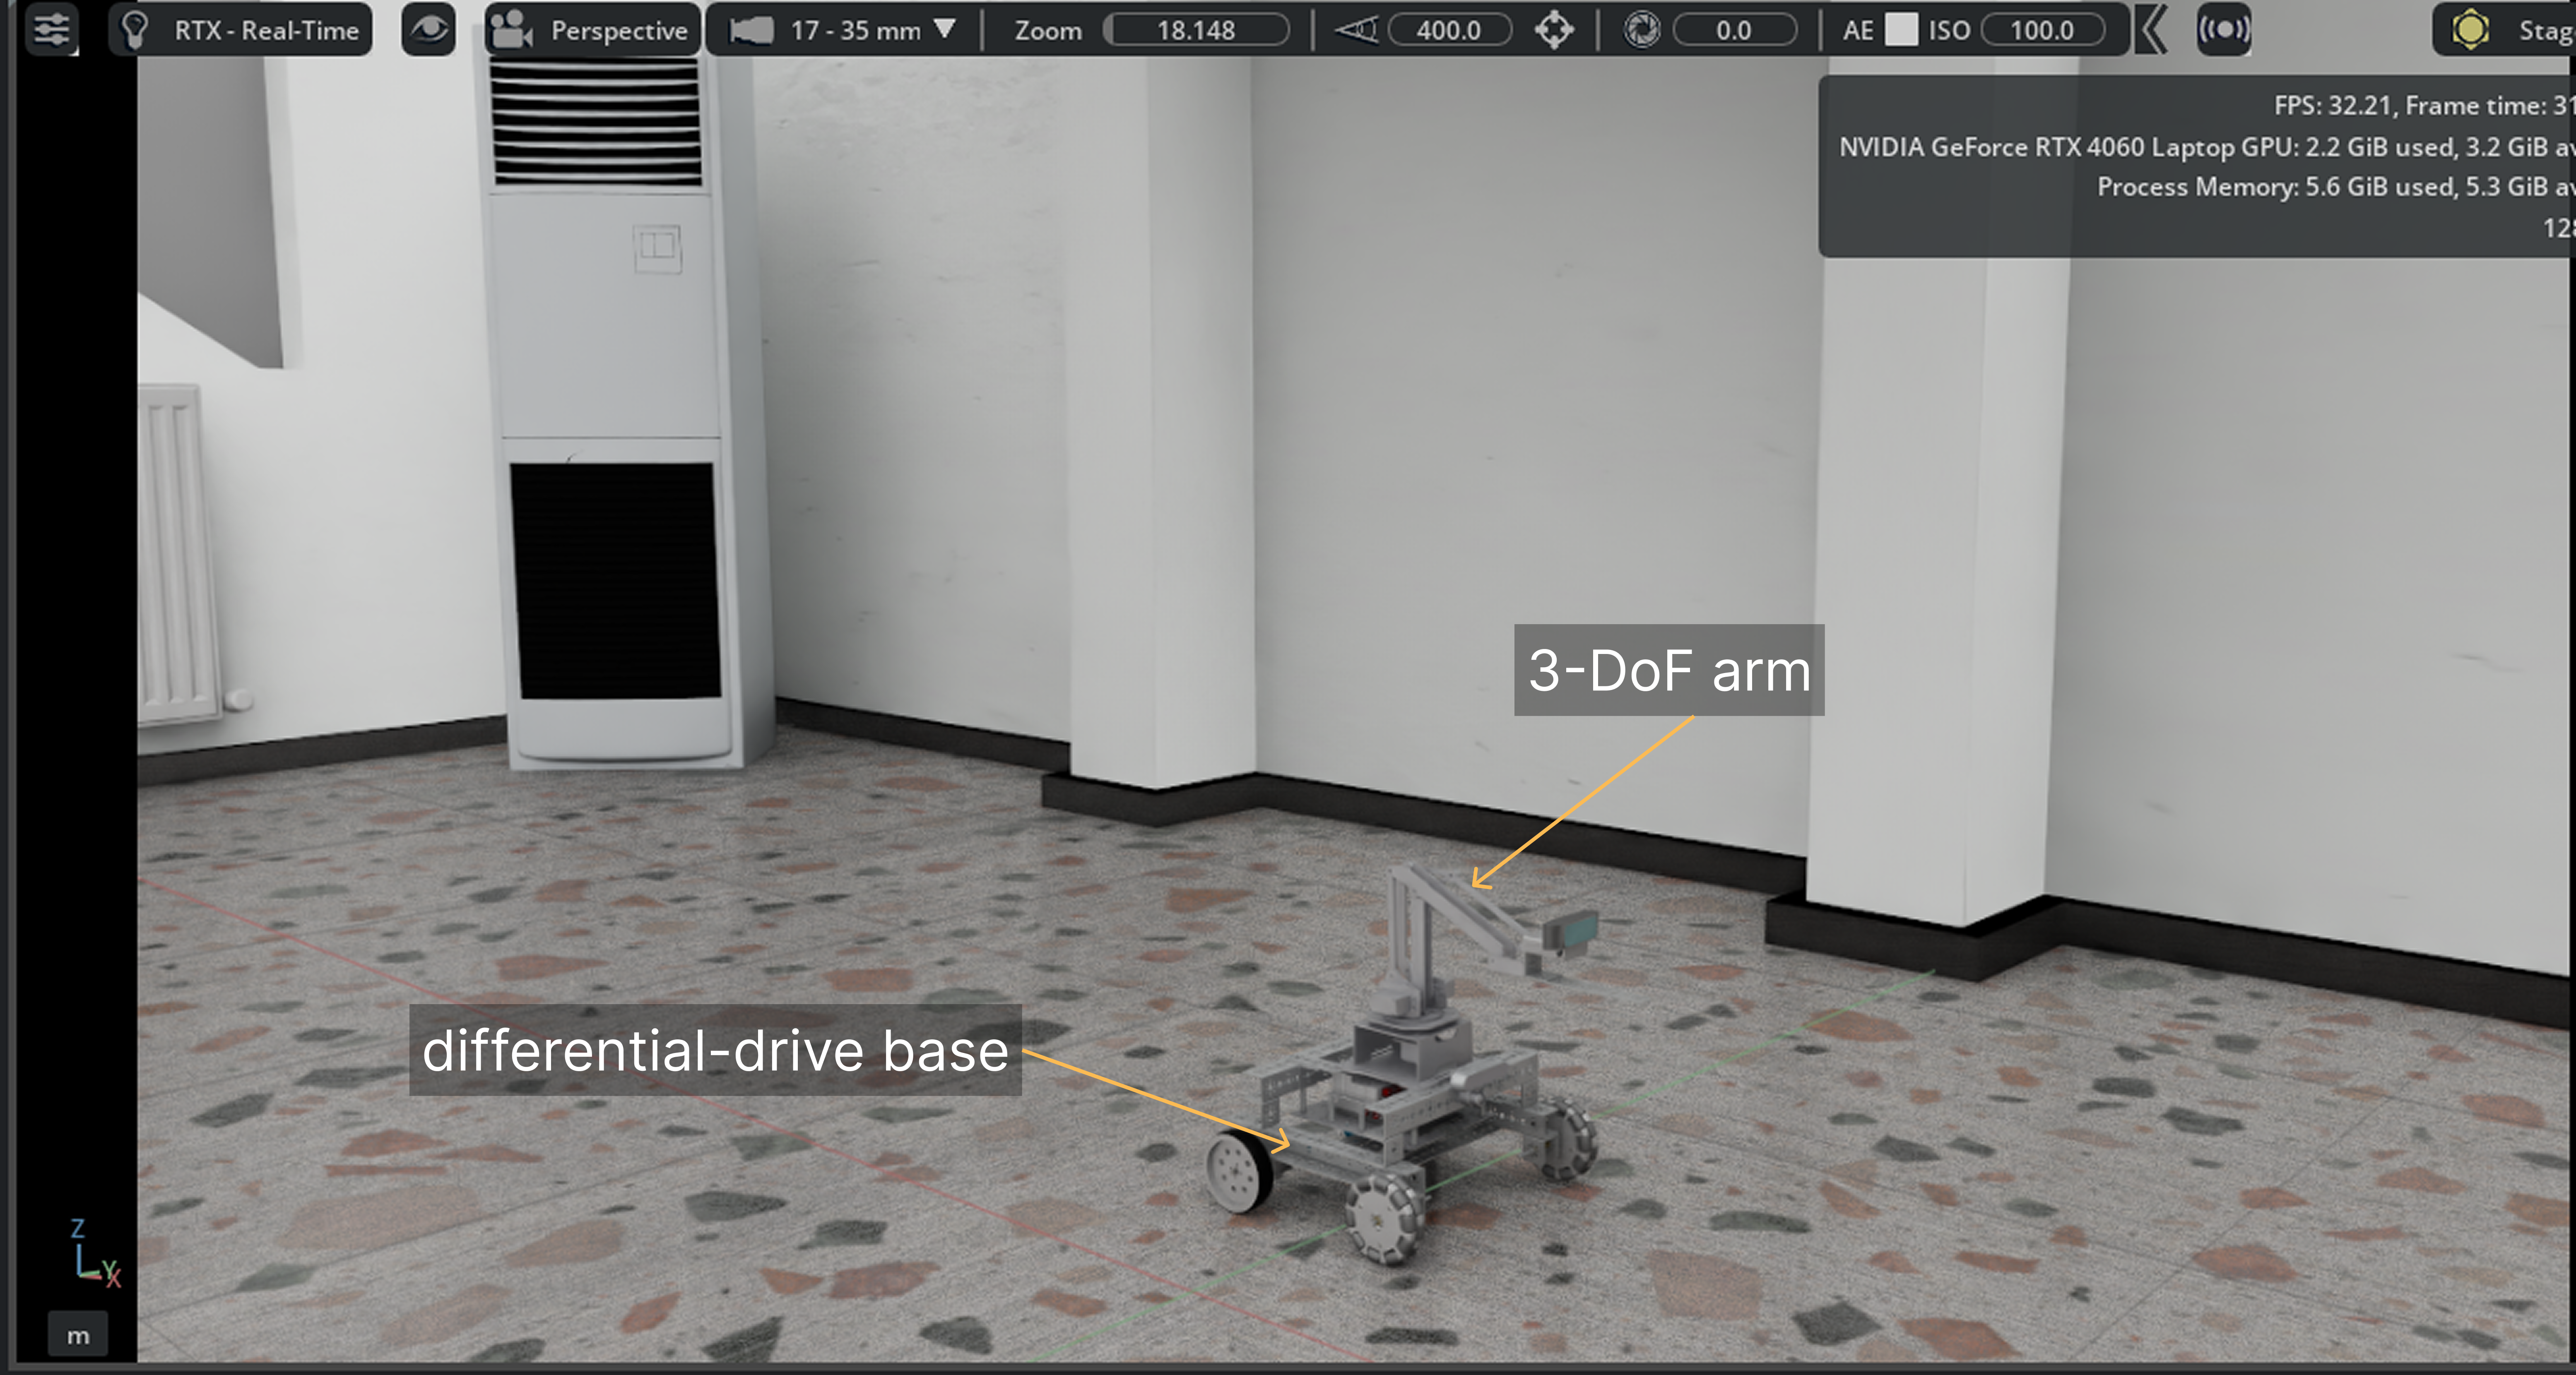
\includegraphics[width=0.72\textwidth]{Figures/report/mech_platform_overview.png}
\caption{Overview of the mobile-manipulator platform and its four subsystems.}
\label{fig:mech_platform_overview_placeholder}
\end{figure}

\subsubsection{CAD Design and Digital-Twin Development}\label{sec:cad}
Every link was modeled in Blender as a separate mesh and arranged into the parent--child hierarchy of the physical chain. The Phobos add-on exports this tree to URDF, generating the joint hierarchy, link definitions, inertial properties (\texttt{<inertial>} tags), and collision models. The same workflow is used for the base and the arm, producing one consistent description for ROS~2 and the Isaac Sim digital twin.

\begin{figure}[!htbp]
\centering
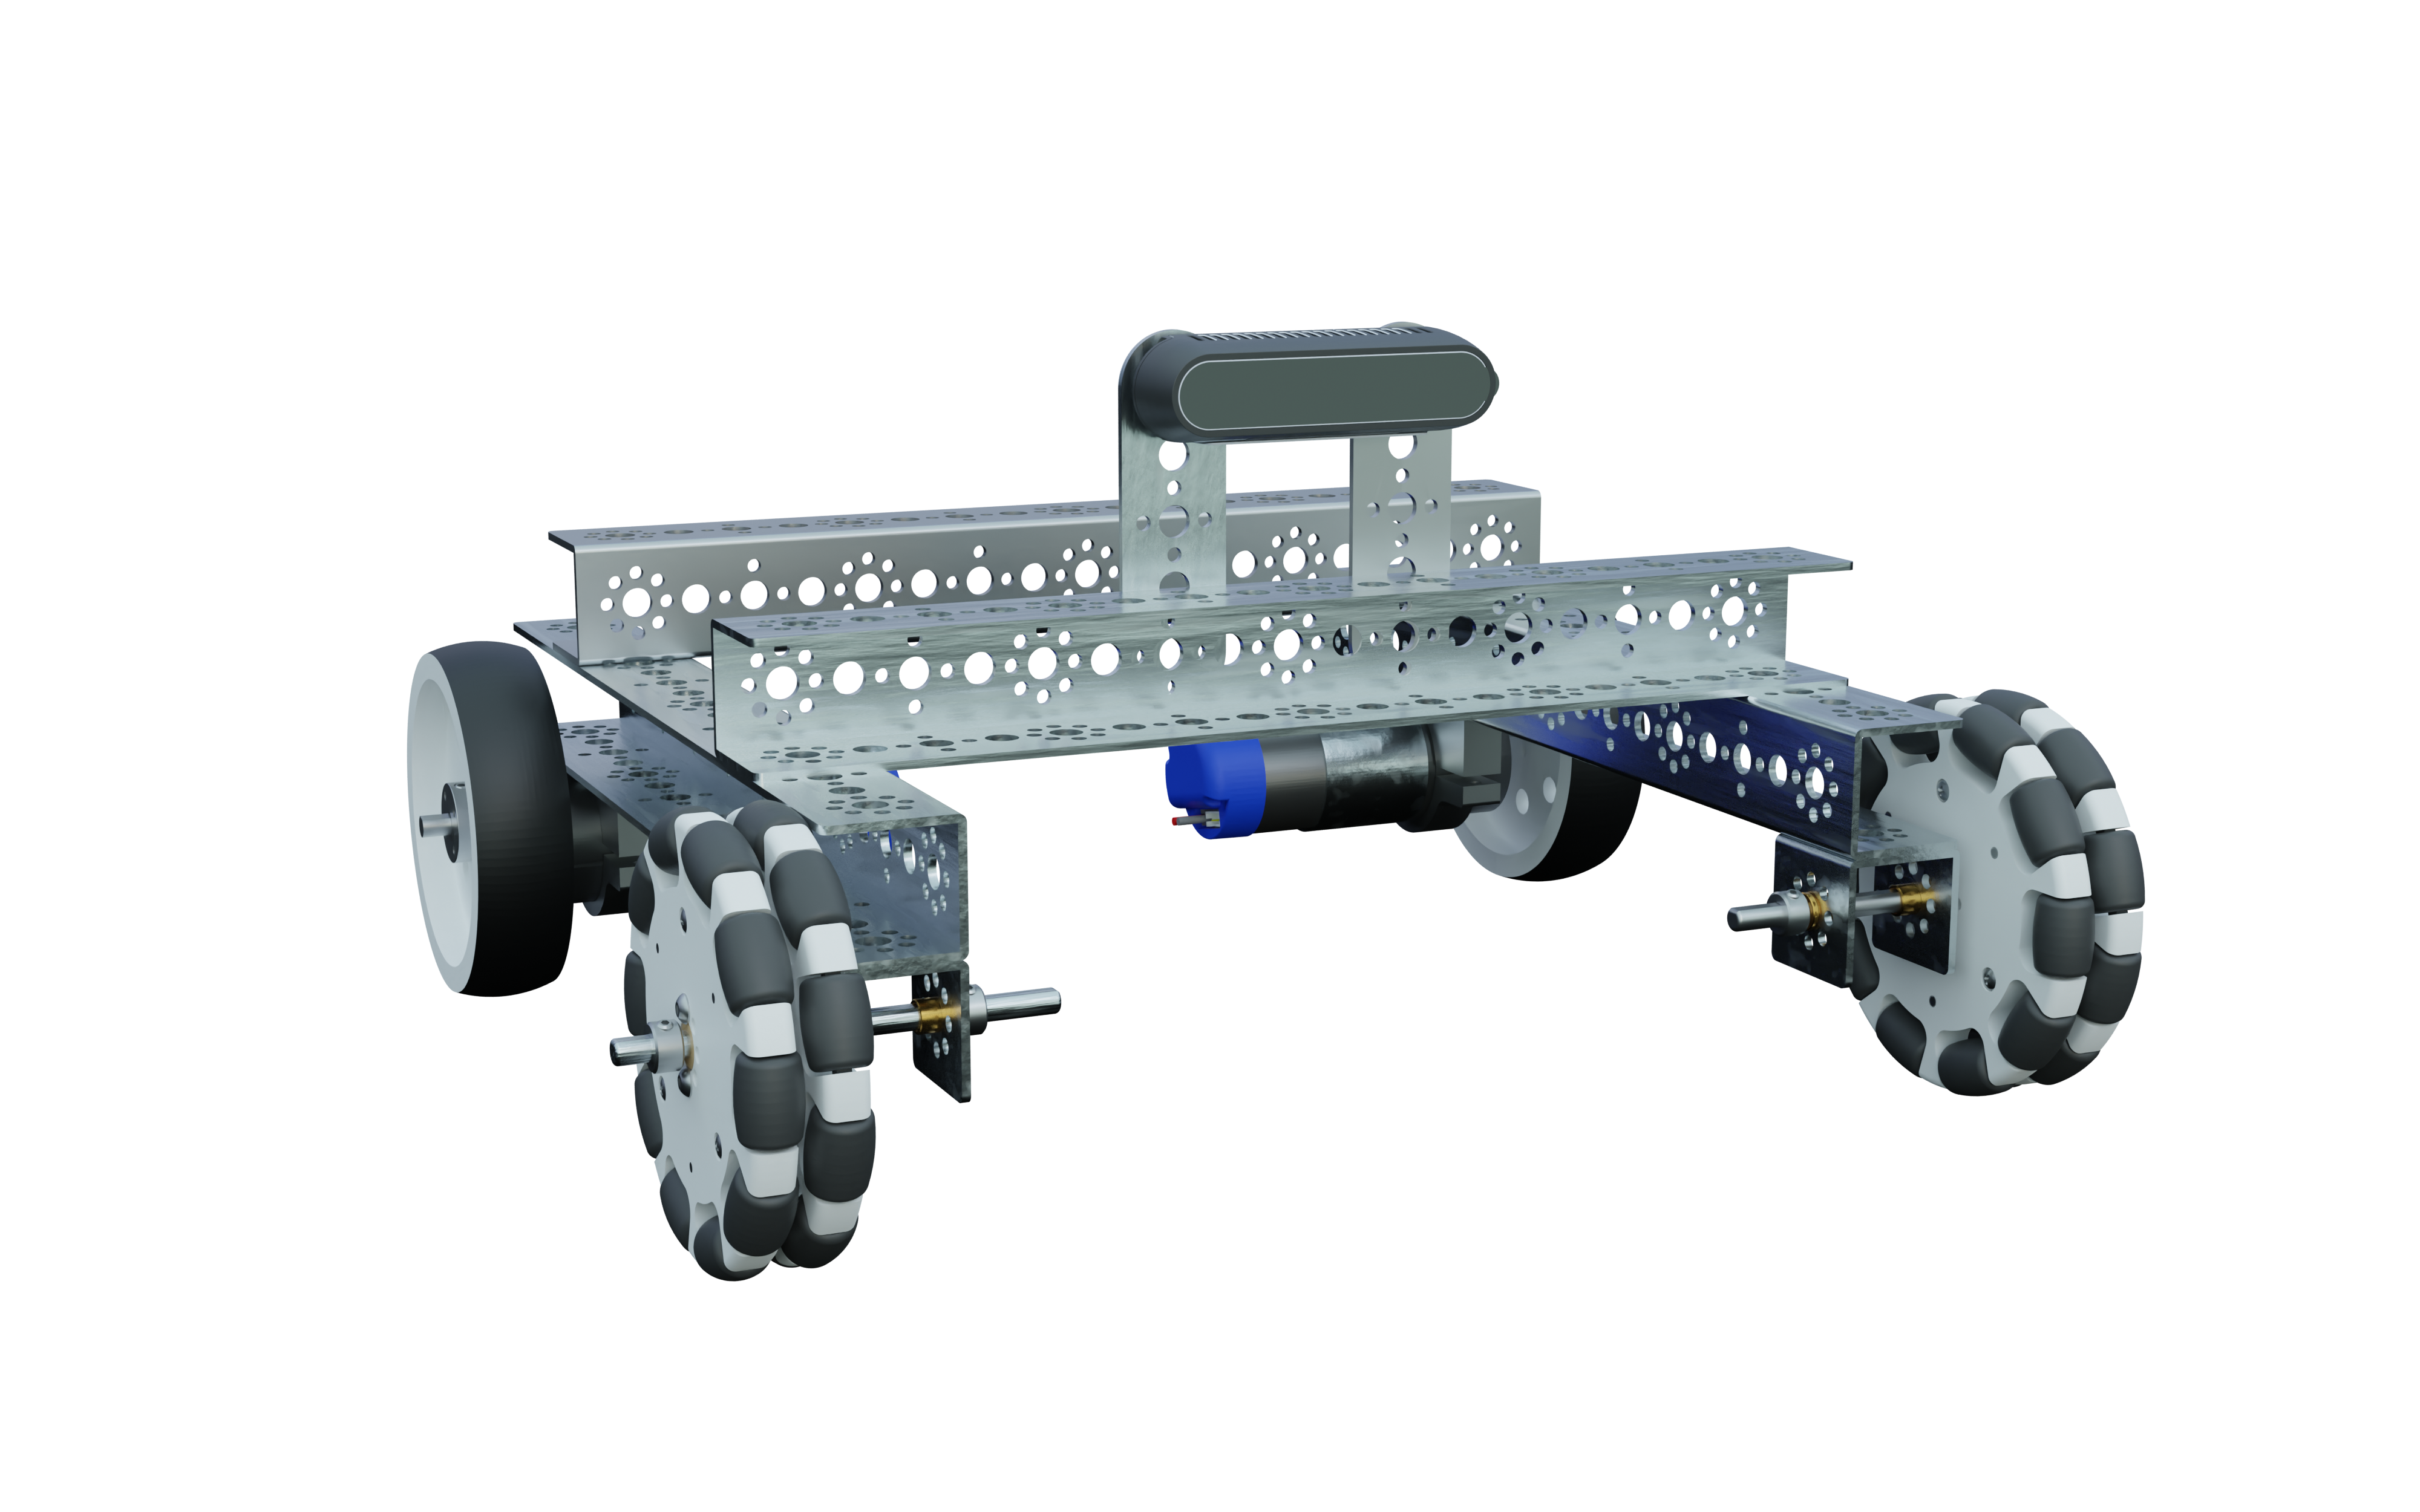
\includegraphics[width=0.82\textwidth]{Figures/blender_model.png}
\caption{Blender--Phobos--URDF pipeline producing the ROS~2 description and the Isaac Sim twin.}
\label{fig:mech_cad_urdf_placeholder}
\end{figure}

\subsubsection{Mobile Robot Mechanical Model}\label{sec:base}
The base is a differential drive. Two independently driven rear wheels set the linear and angular velocity through the sum and difference of their speeds, while passive front omni wheels provide support. The rear wheels are driven by TorqueNADO DC gear-motors, identified in Section~\ref{sec:motorid}. Mass properties are taken from CAD: the volume gives the mass,
\begin{equation}\label{eq:mass}
m=\rho\,V,
\end{equation}
and integration over the solid gives the center of mass and inertia tensor,
\begin{equation}\label{eq:inertia}
\mathbf{r}_c=\frac{1}{m}\int_{\mathcal{B}}\rho\,\mathbf{r}\,\mathrm{d}V,\qquad
\mathbf{I}=\int_{\mathcal{B}}\rho\big(\lVert\mathbf{r}-\mathbf{r}_c\rVert^2\mathbf{1}-(\mathbf{r}-\mathbf{r}_c)(\mathbf{r}-\mathbf{r}_c)^{\!\top}\big)\,\mathrm{d}V,
\end{equation}
with the inertia tensor written explicitly as
\begin{equation}\label{eq:itensor}
\mathbf{I}=\begin{bmatrix} I_{xx}&-I_{xy}&-I_{xz}\\ -I_{xy}&I_{yy}&-I_{yz}\\ -I_{xz}&-I_{yz}&I_{zz}\end{bmatrix}.
\end{equation}
These are written automatically into each link's \texttt{<inertial>} tag. Accurate inertia is essential because simulated acceleration scales inversely with it, so motion prediction and controller tuning both depend on it.

\begin{figure}[!htbp]
\centering
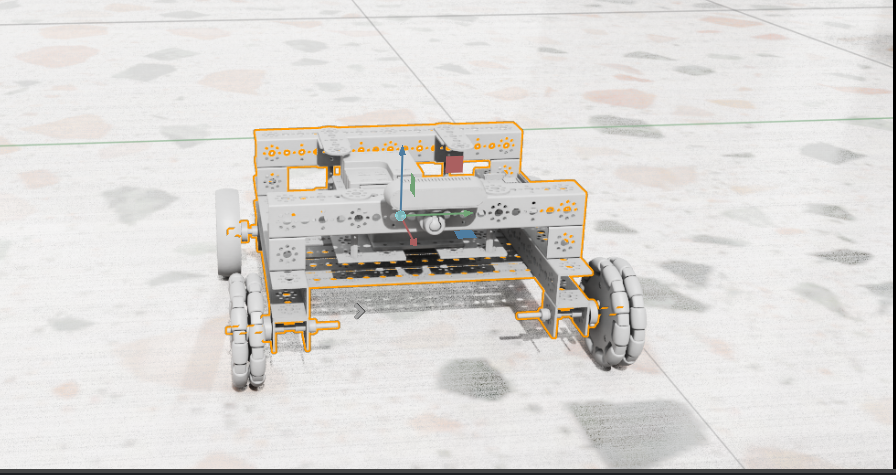
\includegraphics[width=0.88\textwidth]{Figures/report/mech_base_mass.png}
\caption{Mobile-base mass properties extracted from CAD and the differential-drive layout.}
\label{fig:mech_base_mass_placeholder}
\end{figure}

Table~\ref{tab:base_specs} lists the geometric and inertial properties of the mobile base as measured from the composed USD model in Isaac~Sim~5.1 using PhysX auto-computed world bounds. The base is a 2-wheel differential-drive platform: the two rear \texttt{\_9055} wheels are actively driven while the two front \texttt{\_6466} dual-omni wheels act as passive casters. The geometric drive track of 357\,mm represents the physical wheel-centre spacing; the controller's \emph{effective} turn track was calibrated to approximately 560\,mm to compensate for skid during in-place pivots.

\begin{table}[!htbp]
\centering
\caption{Mobile-robot base specifications measured in Isaac~Sim~5.1 (PhysX, USD world bounds).}
\label{tab:base_specs}
\small
\setlength{\tabcolsep}{5pt}
\begin{tabular}{@{}ll@{}}
\toprule
Property & Value \\
\midrule
Base link mass & 4.5\,kg \\
Total robot mass (base + 4 wheels) & 5.164\,kg \\
Dimensions (L\,$\times$\,W\,$\times$\,H) & $300 \times 382 \times 173$\,mm \\
Height span above floor & 25\,mm -- 198\,mm \\
Center of mass (base-link frame) & $(-1.2,\ 0.5,\ 30.9)$\,mm \\
Rear (drive) track, centre-to-centre & 357\,mm \\
Front track & 352\,mm \\
Wheelbase (rear $\to$ front axle) & 237\,mm \\
Effective turn track (calibrated) & $\approx 560$\,mm \\
\bottomrule
\end{tabular}
\end{table}

\begin{table}[!htbp]
\centering
\caption{Wheel specifications of the mobile base.}
\label{tab:wheel_specs}
\small
\setlength{\tabcolsep}{4pt}
\begin{tabular}{@{}llccc@{}}
\toprule
Wheel & Count & Role & Mass (each) & Diameter\,$\times$\,Width \\
\midrule
Rear (\texttt{\_9055})  & 2 & Differential drive       & 0.132\,kg & $101.6 \times 26.4$\,mm \\
Front (\texttt{\_6466}) & 2 & Dual-omni passive caster & 0.200\,kg & $104.8 \times 30.7$\,mm \\
\bottomrule
\end{tabular}
\end{table}

\subsubsection{Collision Modeling}\label{sec:collision}
Visual meshes (high-detail, for rendering) are separated from collision meshes (simplified, for contact). Contact is represented by a signed distance field, negative inside the body and positive outside,
\begin{equation}\label{eq:sdf}
\Phi(\mathbf{x})=\begin{cases}+\,\mathrm{dist}(\mathbf{x},\partial\mathcal{B}) & \mathbf{x}\notin\mathcal{B},\\ -\,\mathrm{dist}(\mathbf{x},\partial\mathcal{B}) & \mathbf{x}\in\mathcal{B},\end{cases}
\end{equation}
whose zero level set is the surface and whose gradient $\nabla\Phi$ is the contact normal. Compared with primitive proxies, the SDF gives continuous collision detection, accurate ground contact, better stability, and less interpenetration. This matters for the wheel--ground, arm--environment, and plug--socket contacts, whose clearances are only millimeters.

\begin{figure}[!htbp]
\centering
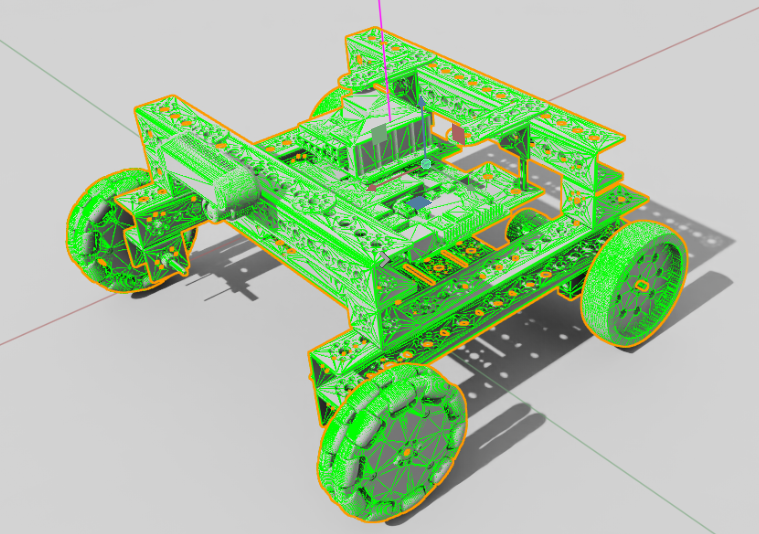
\includegraphics[width=0.88\textwidth]{Figures/report/mech_sdf.png}
\caption{Visual mesh versus the SDF collision representation used in Isaac Sim.}
\label{fig:mech_sdf_placeholder}
\end{figure}

\subsubsection{Manipulator Mechanical Design}\label{sec:manip}
The arm is a 3-DoF serial chain with link lengths
\begin{equation}\label{eq:dims}
L_0=\mechSI{84.4}{mm},\ L_1=\mechSI{8.14}{mm},\ L_2=\mechSI{128.4}{mm},\ L_3=\mechSI{138.0}{mm},\ L_4=\mechSI{16.8}{mm}.
\end{equation}
Because $L_1$ and $L_4$ are horizontal offsets in the plane of motion they enter only as their sum,
\begin{equation}\label{eq:r0}
r_0=L_1+L_4=\mechSI{24.94}{mm}.
\end{equation}
Joint~1 is base yaw, Joint~2 shoulder pitch, Joint~3 elbow pitch. A fourth, passive wrist is mechanically coupled to the two pitch joints,
\begin{equation}\label{eq:passive}
\theta_{3,\text{passive}}=270^{\circ}-\theta_1-\theta_2-90^{\circ}=180^{\circ}-\theta_1-\theta_2,
\end{equation}
where the fixed $270^{\circ}$ and $90^{\circ}$ terms are the constant offsets set by the linkage geometry. This coupling keeps the plug level (fixed orientation) as the arm reconfigures, so the mechanism has three controllable DoF despite four moving joints.
The passive wrist is realized as a planar four-link mechanism that mechanically couples the wrist
to the shoulder and elbow motions. As the two active pitch joints rotate, the linkage drives the
final link so that the plug mounting plate remains approximately level throughout the motion.
This removes the need for a fourth actuator while preserving the orientation constraint required
for plug--socket alignment in the laboratory charging task.

\begin{figure}[t]
\centering
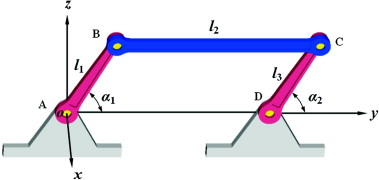
\includegraphics[width=0.82\textwidth]{Figures/report/passive_wrist_fourlink.png}
\caption{Passive wrist implemented as a four-link mechanism that preserves the plug orientation
while the shoulder and elbow joints move.}
\label{fig:passive_wrist_fourlink}
\end{figure}
\begin{figure}[!htbp]
\centering
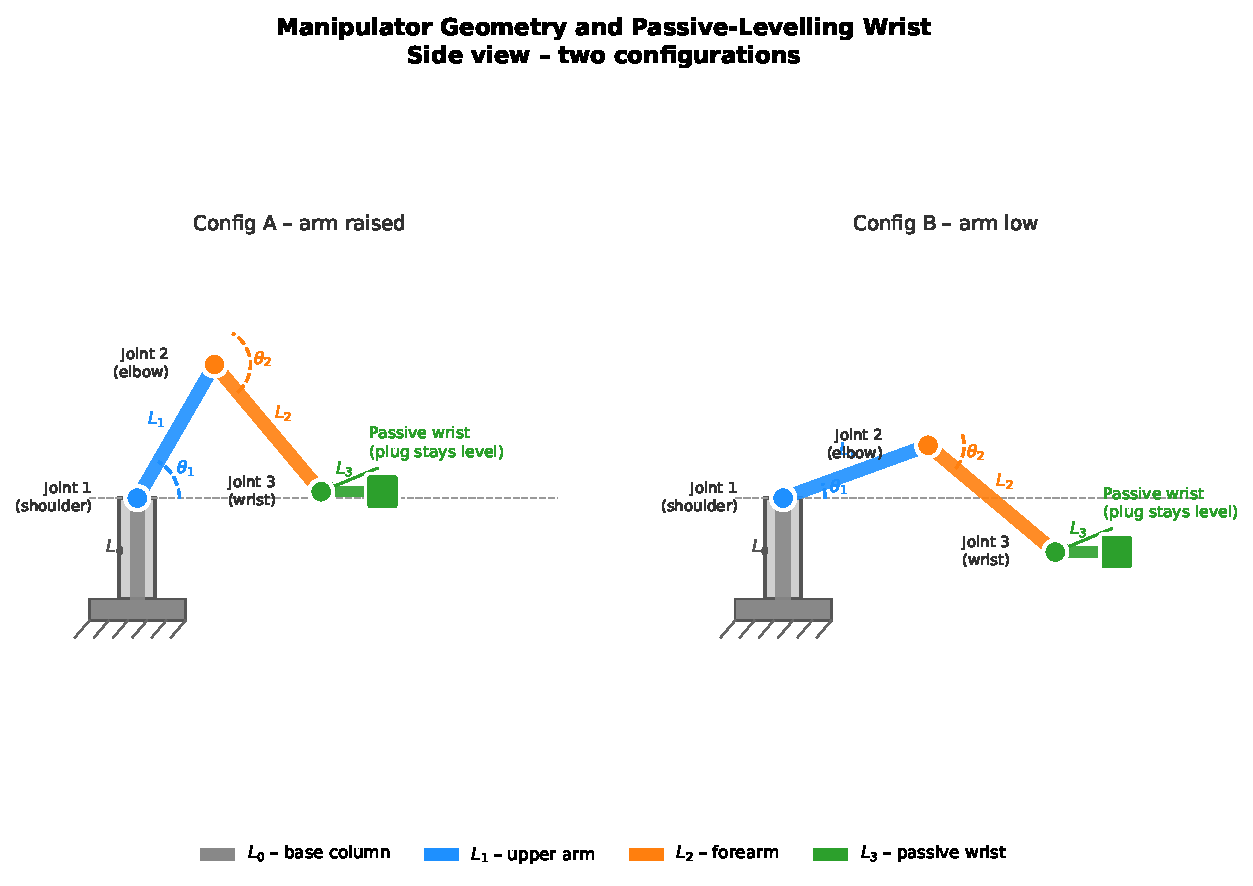
\includegraphics[width=0.88\textwidth]{Figures/report/fig_arm_geometry.png}
\caption{Manipulator geometry, link lengths, and the passive leveling wrist.}
\label{fig:mech_arm_geometry_placeholder}
\end{figure}



\subsubsection{Forward Kinematics}\label{sec:fk}
Composing homogeneous transforms along the chain (with $c_i=\cos\theta_i,\ s_i=\sin\theta_i$),
\begin{equation}\label{eq:T01}
T_{01}=R_z(\theta_1)\,\mathrm{Trans}(r_0,0,L_0)=
\begin{bmatrix} c_1&-s_1&0&r_0c_1\\ s_1&c_1&0&r_0s_1\\ 0&0&1&L_0\\ 0&0&0&1\end{bmatrix},
\end{equation}
\begin{equation}\label{eq:T12}
\begin{aligned}
T_{12}&=R_y(\theta_2)\,\mathrm{Trans}(0,0,L_2)=
\begin{bmatrix} c_2&0&s_2&L_2s_2\\ 0&1&0&0\\ -s_2&0&c_2&L_2c_2\\ 0&0&0&1\end{bmatrix},\\[4pt]
T_{23}&=R_y(\theta_3)\,\mathrm{Trans}(0,0,L_3)=
\begin{bmatrix} c_3&0&s_3&L_3s_3\\ 0&1&0&0\\ -s_3&0&c_3&L_3c_3\\ 0&0&0&1\end{bmatrix}.
\end{aligned}
\end{equation}
The passive-wrist transform $T_{34}=R_y(\theta_{3,\text{passive}})$ acts at the wrist origin and does not move it. Multiplying the three transforms $T_{01}T_{12}T_{23}$ and reading off the translation column gives the closed-form wrist position
\begin{equation}\label{eq:fk}
\boxed{\;
\begin{aligned}
\rho(\theta_2,\theta_3)&=r_0+L_2\sin\theta_2+L_3\sin(\theta_2+\theta_3),\\
x&=\rho\cos\theta_1,\qquad y=\rho\sin\theta_1,\\
z(\theta_2,\theta_3)&=L_0+L_2\cos\theta_2+L_3\cos(\theta_2+\theta_3).
\end{aligned}\;}
\end{equation}
Here $\rho$ is the radial reach (shoulder and elbow projections plus the offset $r_0$), $z$ the height, and the base yaw $\theta_1$ only rotates that reach into $x,y$. This closed form equals the full transform product exactly.

\begin{figure}[!htbp]
\centering
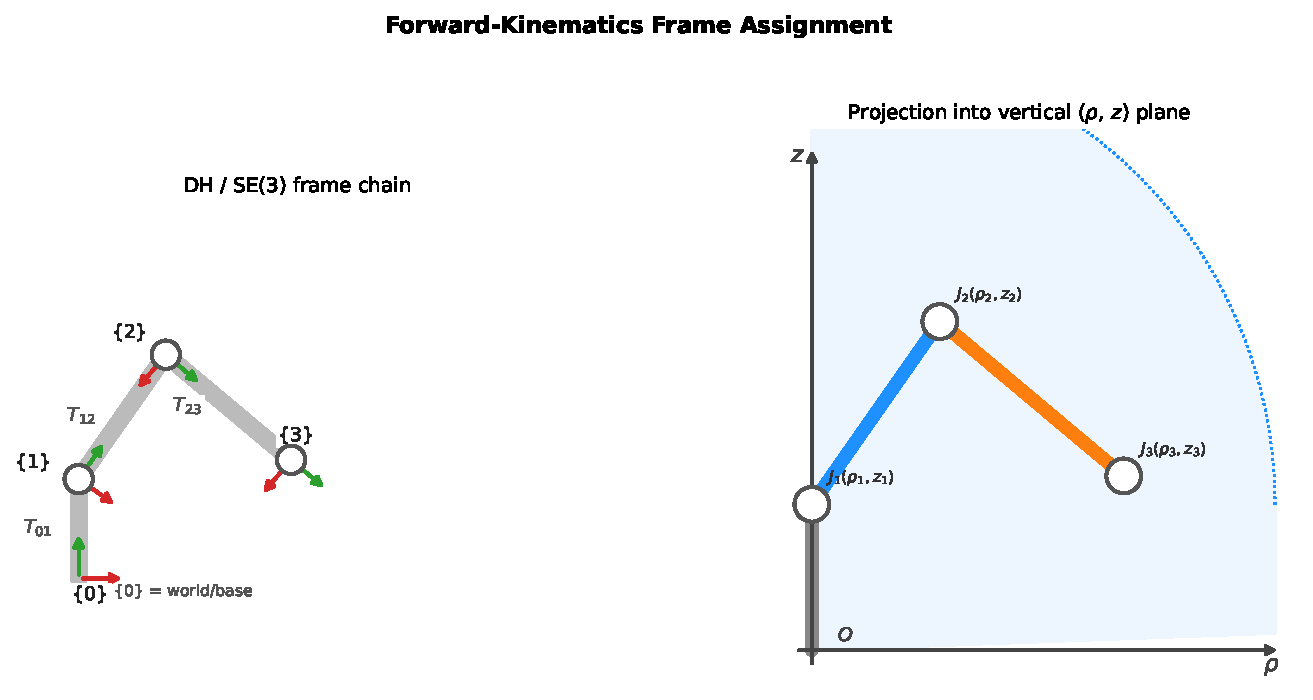
\includegraphics[width=0.88\textwidth]{Figures/report/fig_fk_frames.png}
\caption{Frame assignment and the planar $(\rho,z)$ projection used in the forward kinematics.}
\label{fig:mech_fk_frames_placeholder}
\end{figure}

\subsubsection{Inverse Kinematics}\label{sec:ik}
The base yaw is set by the target azimuth,
\begin{equation}\label{eq:ik1}
\theta_1=\operatorname{atan2}(y_d,x_d),
\end{equation}
and the planar wrist coordinates relative to the shoulder are
\begin{equation}\label{eq:ikuw}
u=\sqrt{x_d^2+y_d^2}-r_0,\qquad w=z_d-L_0.
\end{equation}
The law of cosines on the triangle $(L_2,L_3,D)$ with $D=\sqrt{u^2+w^2}$ gives the elbow,
\begin{equation}\label{eq:ikelbow}
\theta_3=\mp\arccos\!\left(\frac{u^2+w^2-L_2^2-L_3^2}{2L_2L_3}\right),
\end{equation}
the two signs being elbow-up and elbow-down, and the shoulder follows as
\begin{equation}\label{eq:ik2}
\theta_2=\operatorname{atan2}(u,w)-\operatorname{atan2}\!\big(L_3\sin\theta_3,\,L_2+L_3\cos\theta_3\big).
\end{equation}
Round-tripping through the forward map over $5\times10^4$ targets gave a worst error of $1.4\times10^{-16}\,\mathrm{m}$. Singularities occur at full extension/folding ($D=L_2+L_3$ or $|L_2-L_3|$) and on the base axis; the reachable shell is $|L_2-L_3|\le D\le L_2+L_3$, i.e.\ $\mechSI{9.6}{mm}\le D\le\mechSI{266.4}{mm}$.

\begin{figure}[!htbp]
\centering
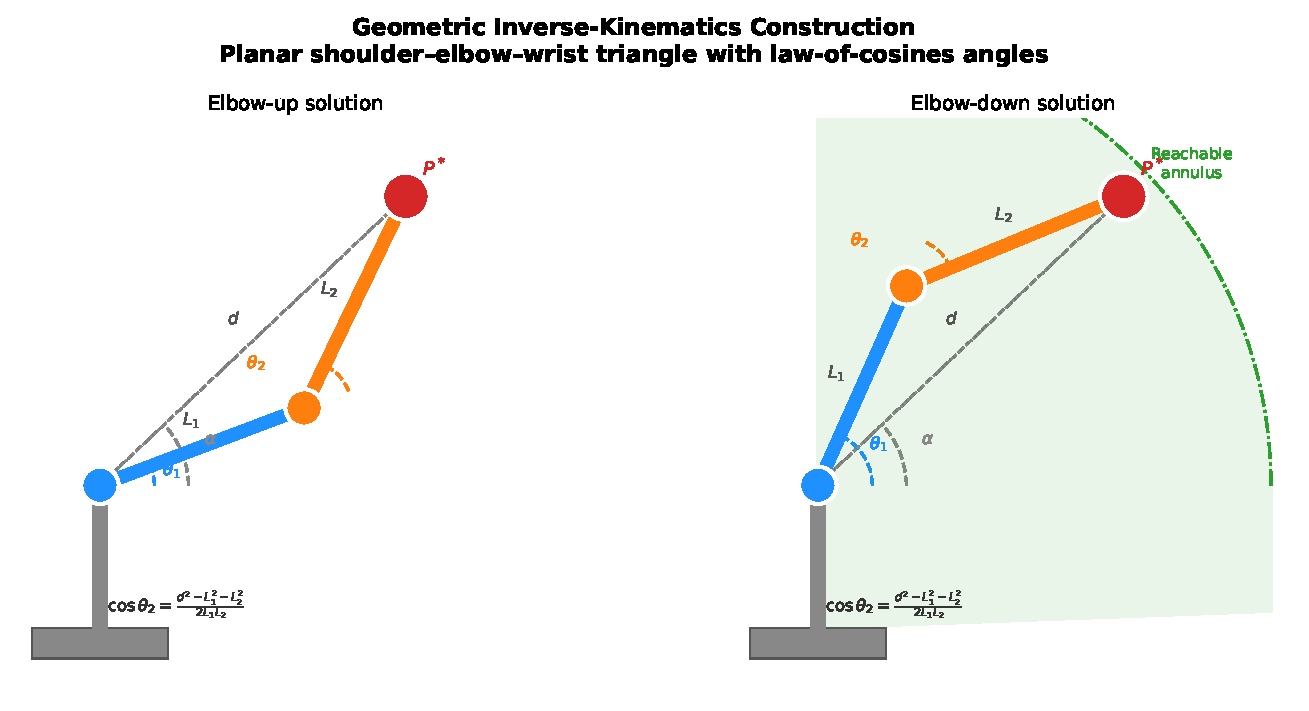
\includegraphics[width=0.88\textwidth]{Figures/report/fig_ik_geometry.png}
\caption{Geometric inverse kinematics: law-of-cosines construction and the two elbow branches.}
\label{fig:mech_ik_geometry_placeholder}
\end{figure}

\subsubsection{Jacobian Analysis}\label{sec:jac}
Differentiating the forward map, $\dot{\mathbf{p}}=J(\mathbf{q})\dot{\mathbf{q}}$ with ($c_{23}=\cos(\theta_2+\theta_3),\ s_{23}=\sin(\theta_2+\theta_3)$)
\begin{equation}\label{eq:jac}
J(\mathbf{q})=\begin{bmatrix}
-\rho s_1 & c_1(L_2c_2+L_3c_{23}) & c_1L_3c_{23}\\
\rho c_1 & s_1(L_2c_2+L_3c_{23}) & s_1L_3c_{23}\\
0 & -(L_2s_2+L_3s_{23}) & -L_3s_{23}\end{bmatrix}.
\end{equation}
Its determinant evaluates to
\begin{equation}\label{eq:detj}
\det J(\mathbf{q})=\rho\,L_2L_3\sin\theta_3,
\end{equation}
so the arm is singular when $\sin\theta_3=0$ (elbow straight/folded) or $\rho=0$ (wrist on the base axis). Because $J$ is square, the manipulability measure reduces to the absolute determinant,
\begin{equation}\label{eq:manip}
\mu=\sqrt{\det(JJ^\top)}=|\det J|=\rho\,L_2L_3|\sin\theta_3|,
\end{equation}
maximal near $\theta_3=\pm90^{\circ}$ and zero at singularities, where positioning sensitivity is worst.

\begin{figure}[!htbp]
\centering
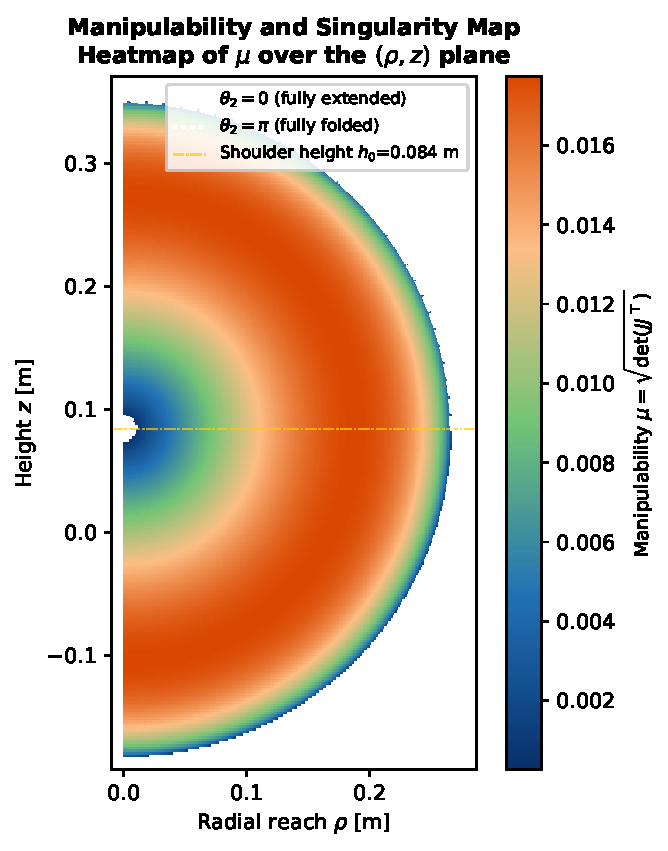
\includegraphics[width=0.82\textwidth]{Figures/report/fig_manipulability.png}
\caption{Manipulability distribution and singular configurations of the manipulator.}
\label{fig:mech_manipulability_placeholder}
\end{figure}

\subsubsection{Dynamic Modeling}\label{sec:dyn}
For the gravity-loaded planar two-link subsystem (shoulder $\theta_1$, elbow $\theta_2$; $l_1=L_2,\ l_2=L_3$), the Euler--Lagrange equations give
\begin{equation}\label{eq:eom}
M(\mathbf{q})\ddot{\mathbf{q}}+C(\mathbf{q},\dot{\mathbf{q}})\dot{\mathbf{q}}+G(\mathbf{q})=\boldsymbol{\tau},
\end{equation}
with the inertia matrix
\begin{equation}\label{eq:M}
M(\mathbf{q})=\begin{bmatrix}
I_1+I_2+m_1l_{c1}^2+m_2(l_1^2+l_{c2}^2+2l_1l_{c2}\cos\theta_2) & I_2+m_2(l_{c2}^2+l_1l_{c2}\cos\theta_2)\\
I_2+m_2(l_{c2}^2+l_1l_{c2}\cos\theta_2) & I_2+m_2l_{c2}^2\end{bmatrix},
\end{equation}
the Coriolis/centrifugal matrix
\begin{equation}\label{eq:C}
C(\mathbf{q},\dot{\mathbf{q}})=\begin{bmatrix} h\dot\theta_2 & h(\dot\theta_1+\dot\theta_2)\\ -h\dot\theta_1 & 0\end{bmatrix},\qquad h=-m_2l_1l_{c2}\sin\theta_2,
\end{equation}
and the gravity vector
\begin{equation}\label{eq:G}
G(\mathbf{q})=\begin{bmatrix} (m_1l_{c1}+m_2l_1)g\cos\theta_1+m_2l_{c2}g\cos(\theta_1+\theta_2)\\ m_2l_{c2}g\cos(\theta_1+\theta_2)\end{bmatrix}.
\end{equation}
The diagonal of $M$ is the effective inertia at each joint, and the off-diagonal entries are the inter-joint coupling; both scale with $\cos\theta_2$. The matrix $C$ holds the velocity-dependent torques. The vector $G$ is the gravity hold-torque, which is largest with a link horizontal and reaches $\approx\mechSI{0.4}{N.m}$ at the shoulder when fully extended. The passive wrist adds no equation: its mass, inertia, and gravity term are reflected into the shoulder and elbow through the coupling, so two dynamic equations describe all four moving bodies.

\begin{figure}[!htbp]
\centering
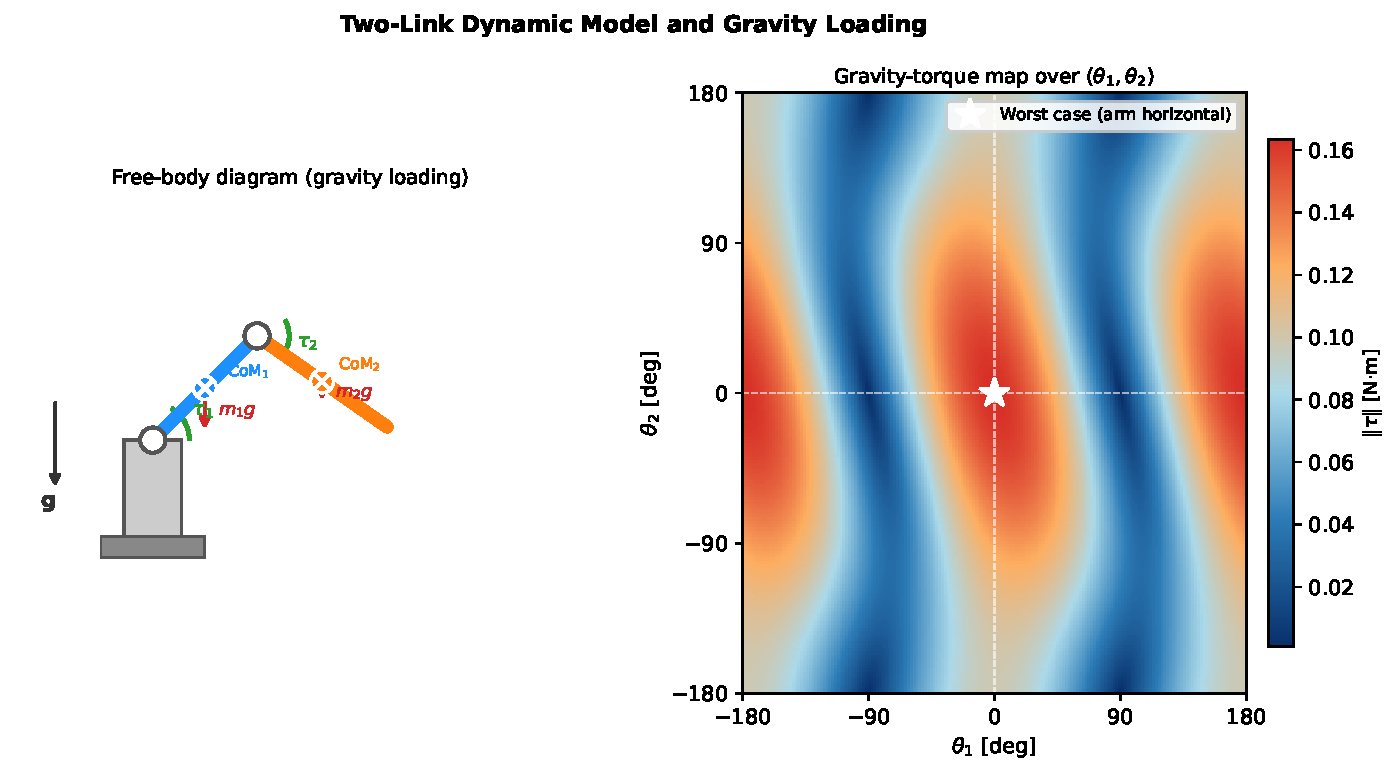
\includegraphics[width=0.88\textwidth]{Figures/report/fig_dynamics.png}
\caption{Two-link dynamic model and the configuration-dependent gravity load.}
\label{fig:mech_dynamics_placeholder}
\end{figure}

\subsubsection{Joint Characterization Experiments}\label{sec:jointid}
Each servo joint is a second-order system,
\begin{equation}\label{eq:jointmodel}
J\ddot\theta+b\dot\theta+k\theta=\tau.
\end{equation}
Four experiments identify the inertia $J$, damping $b$, and stiffness $k$: a step response, a free oscillation, a frequency sweep, and a static deflection test.

\textbf{Experiment 1: Step response.} The ESP32 commands a position step and streams $(t,\theta)$; the data is Savitzky--Golay smoothed and fitted to the full second-order step response
\begin{equation}\label{eq:stepform}
\theta(t)=\theta_0+(\theta_f-\theta_0)\,g(t),
\end{equation}
with $g(t)$ underdamped, critically damped, or overdamped,
\begin{equation}\label{eq:gforms}
g_{\zeta<1}=1-e^{-\zeta\omega_n t}\!\Big[\cos\omega_d t+\tfrac{\zeta}{\sqrt{1-\zeta^2}}\sin\omega_d t\Big],\quad
g_{\zeta=1}=1-e^{-\omega_n t}(1+\omega_n t),\quad
g_{\zeta>1}=1+\tfrac{s_1e^{s_2t}-s_2e^{s_1t}}{s_2-s_1},
\end{equation}
where $\omega_d=\omega_n\sqrt{1-\zeta^2}$ and $s_{1,2}=-\omega_n(\zeta\mp\sqrt{\zeta^2-1})$. The parameters $(\theta_0,\theta_f,\zeta,\omega_n)$ minimize
\begin{equation}\label{eq:lscost}
\mathcal{J}=\frac{1}{N}\sum_{k=1}^{N}\big[\theta_{\text{meas}}(t_k)-\theta(t_k)\big]^2
\end{equation}
by multi-start Nelder--Mead. With the inertia $J$ known, the stiffness and damping follow:
\begin{equation}\label{eq:kb}
k=J\,\omega_n^2,\qquad b=2\zeta J\omega_n.
\end{equation}

\textbf{Experiment 2: Free oscillation.} An unpowered release decays as $\theta=\theta_0e^{-\zeta\omega_n t}\cos(\omega_d t+\varphi)$; the logarithmic decrement gives the damping,
\begin{equation}\label{eq:logdec}
\delta=\ln\frac{x_n}{x_{n+1}},\qquad \zeta=\frac{\delta}{\sqrt{4\pi^2+\delta^2}}.
\end{equation}

\textbf{Experiment 3: Frequency response.} A swept sinusoid yields the Bode plot, giving the resonance frequency, bandwidth, and dynamic stiffness.

\textbf{Experiment 4: Static deflection.} Known torques at zero speed give the stiffness directly,
\begin{equation}\label{eq:static}
k=\frac{\tau}{\Delta\theta},
\end{equation}
and $1/k$ is the compliance that lets the rigid arm absorb small insertion misalignments.

\begin{figure}[!htbp]
\centering
\begin{subfigure}[b]{0.60\textwidth}
  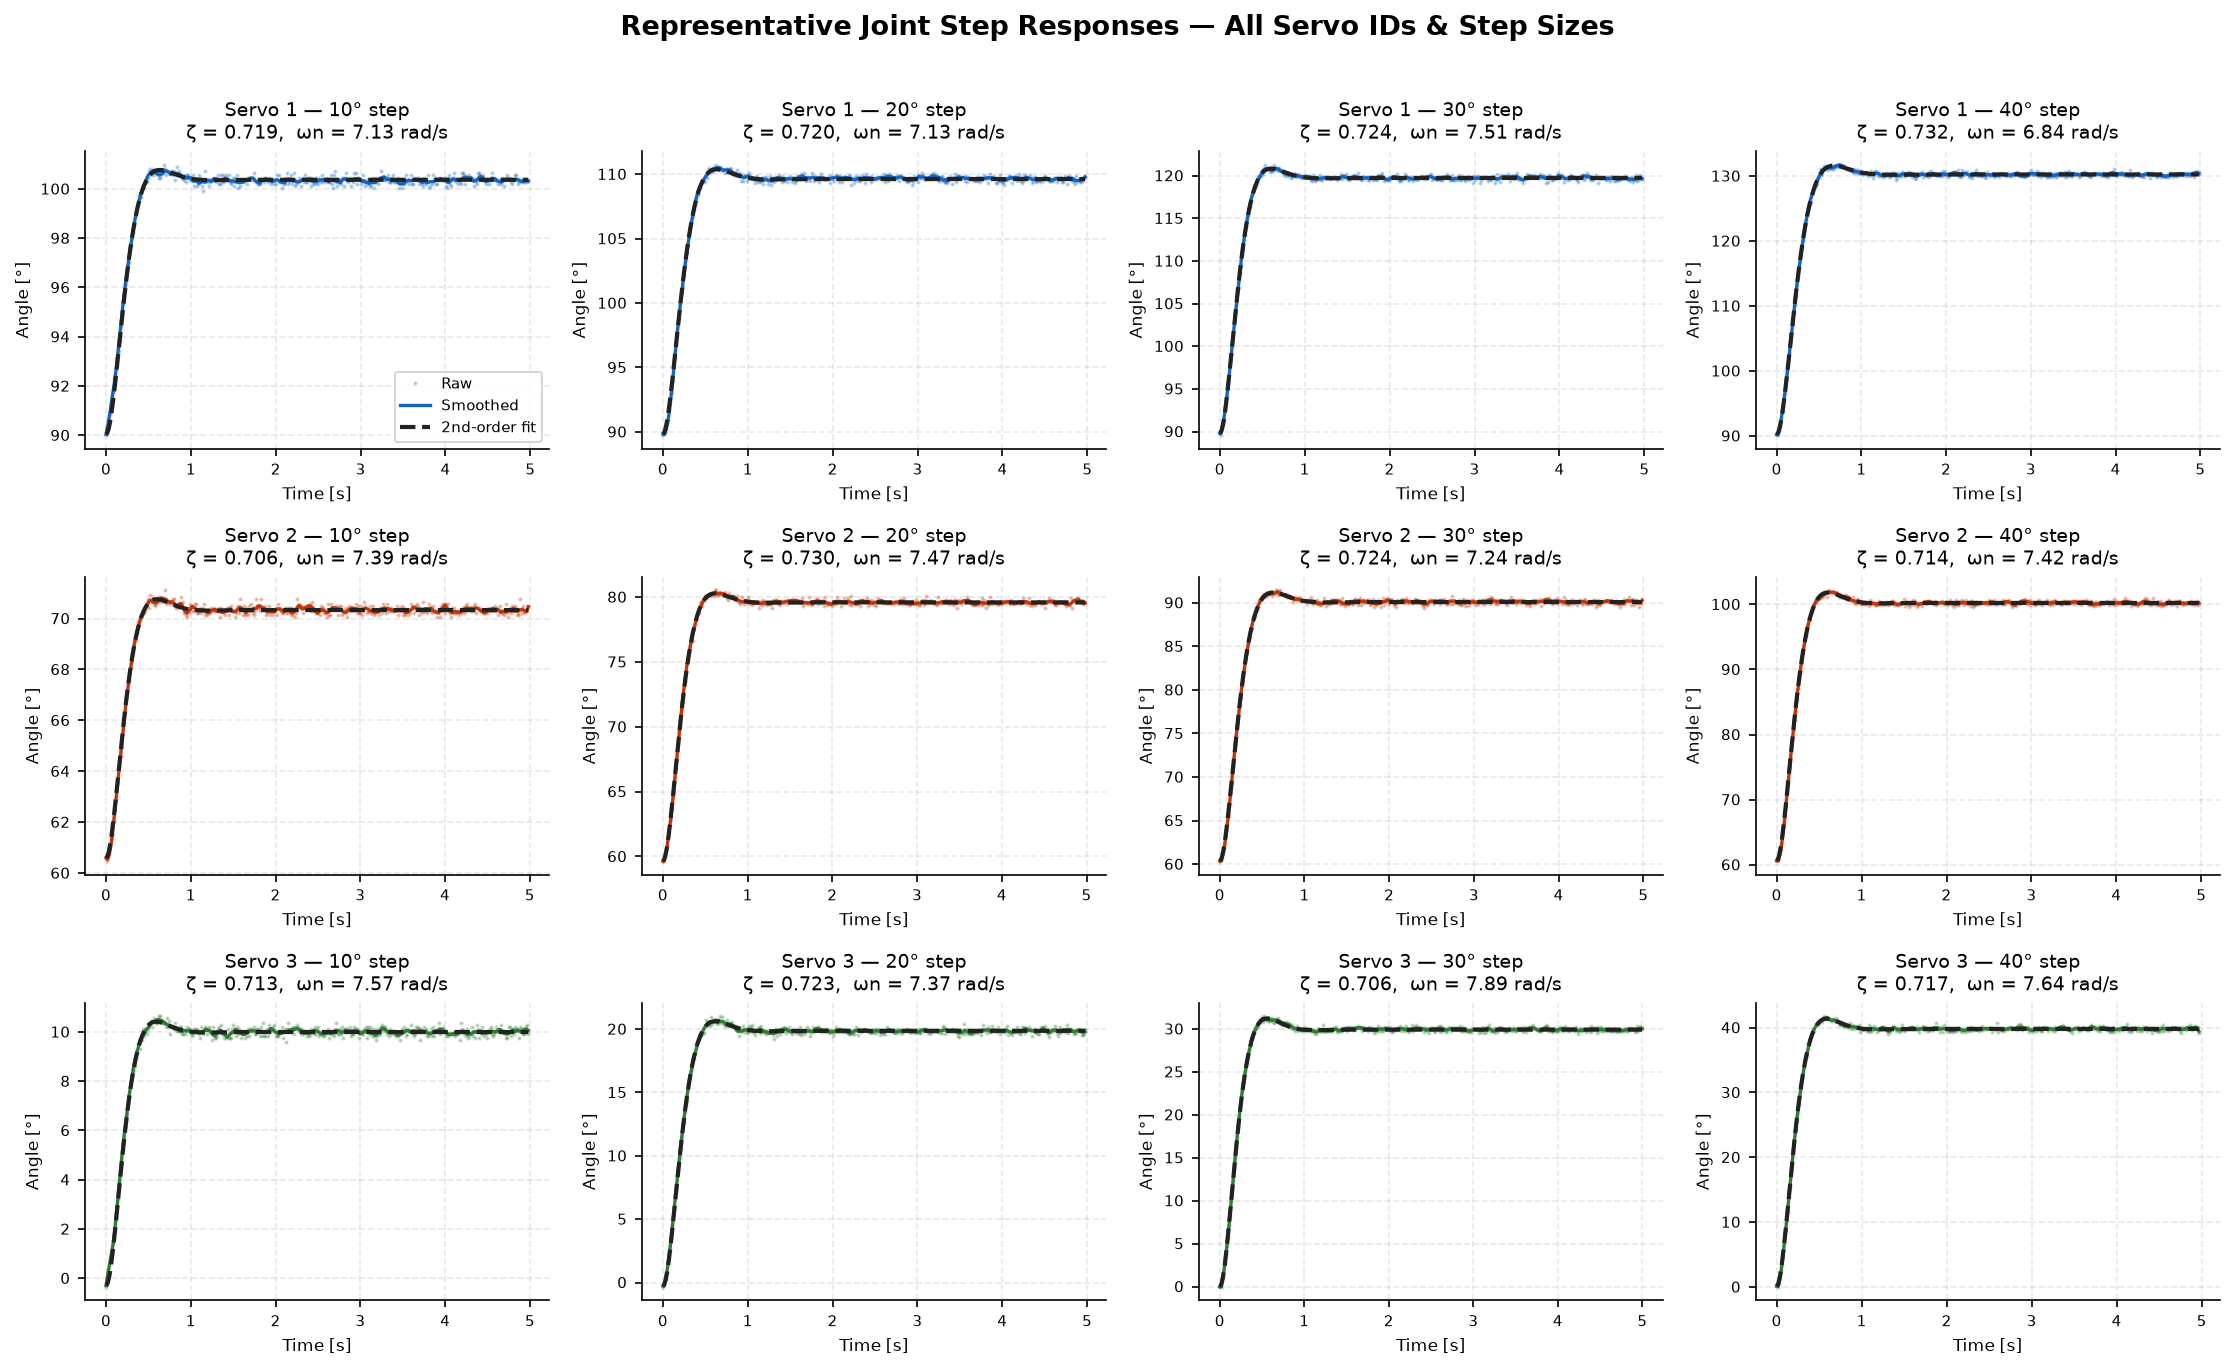
\includegraphics[width=\textwidth]{Figures/report/joint_step_responses.png}
  \caption{Representative step responses with second-order fits.}
\end{subfigure}
\hfill
\begin{subfigure}[b]{0.37\textwidth}
  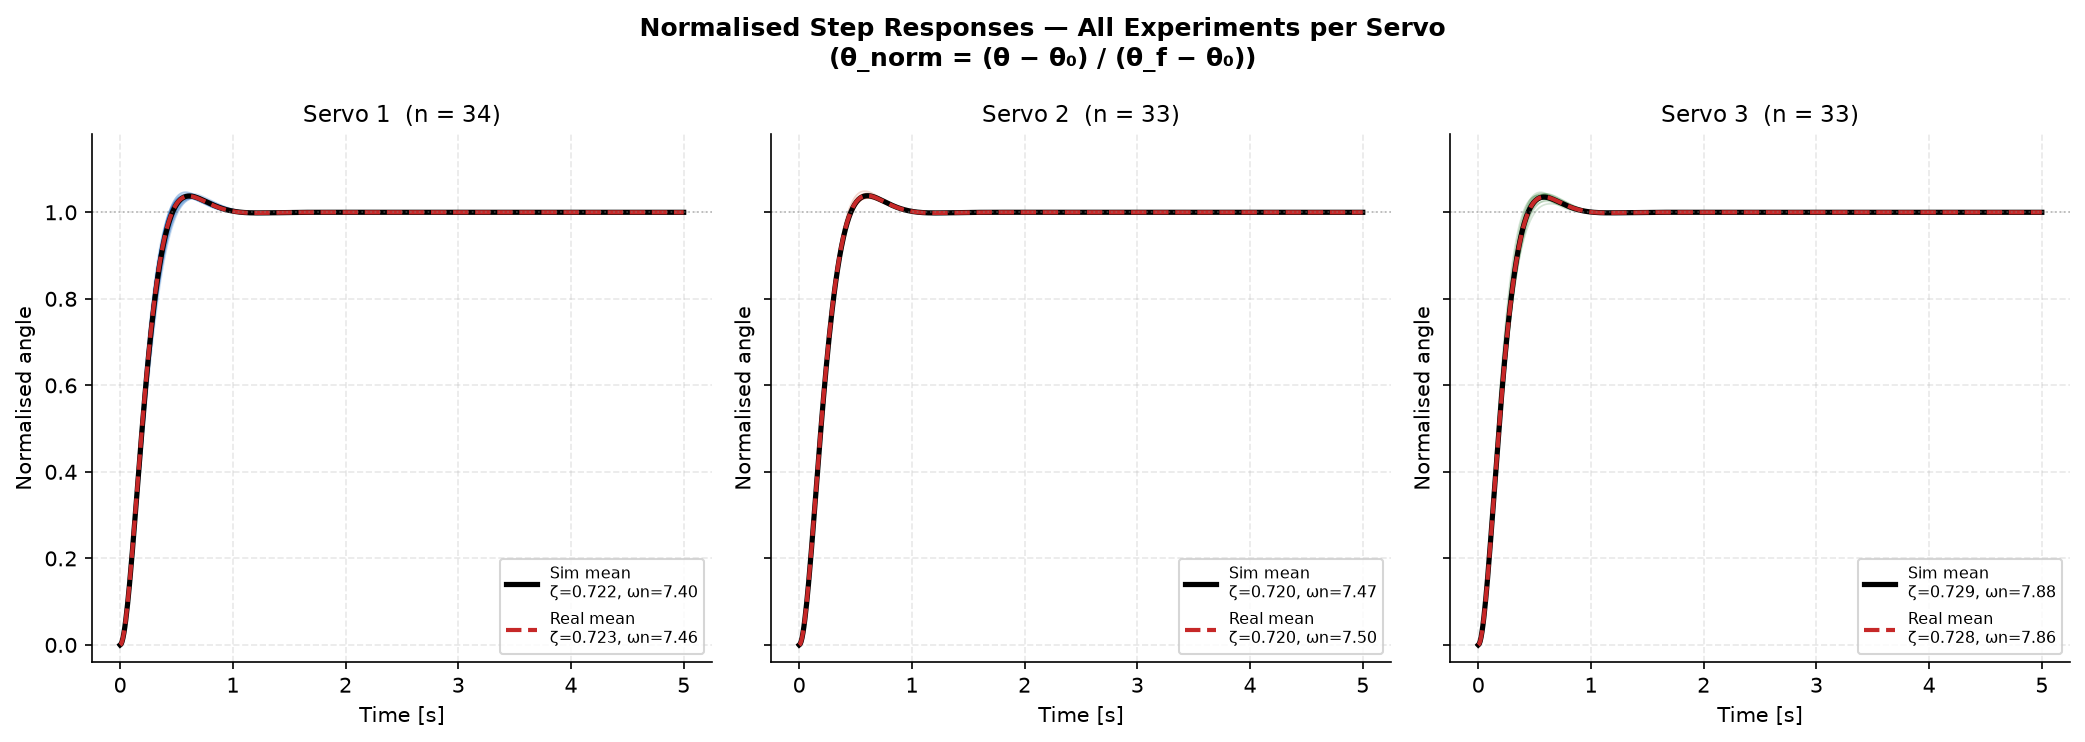
\includegraphics[width=\textwidth]{Figures/report/joint_normalized_fits.png}
  \caption{Normalised fit overlay.}
\end{subfigure}
\caption{Joint identification: step-response fit, free-oscillation decay, and frequency response.}
\label{fig:mech_joint_identification_placeholder}
\end{figure}

\subsubsection{TorqueNADO Motor Parameter Identification}\label{sec:motorid}
The DC drive motor follows
\begin{equation}\label{eq:motoreq}
V=Ri+L\frac{\mathrm di}{\mathrm dt}+K_e\omega,\qquad J\dot\omega=K_ti-b\omega-\tau_L.
\end{equation}
\textbf{Scenario 1 (no-load steady state):} $V=Ri+K_e\omega$ solved by least squares $\hat{\boldsymbol\theta}=(\Phi^\top\Phi)^{-1}\Phi^\top\mathbf{y}$ gives $R=\mechSI{16}{\Omega}$, $K_e=0.013178~\mathrm{V/(rad/s)}$ ($R^2>0.9$).
\textbf{Scenario 2 (coast-down):} $\omega=\omega_0e^{-t/\tau}$, $\ln\omega=\ln\omega_0-t/\tau$ gives $\tau=\mechSI{1.1336}{s}$, $b/J=1/\tau=\mechSI{0.8819}{s^{-1}}$.
\textbf{Scenario 3 (step):} $J\dot\omega\approx K_ti\Rightarrow J=K_ti/\dot\omega=\mechSI{0.001}{kg.m^2}$, then $b=J(b/J)\approx\mechSI{8.82e-4}{N.m.s}$.
\textbf{Scenario 4 (low duty):} $V\approx Ri$ re-confirms $R$.

\begin{table}[htbp]\centering
  \caption{Identified TorqueNADO motor parameters.}\label{tab:motor}
  \small\setlength{\tabcolsep}{5pt}
  \begin{tabular}{@{}llll@{}}
    \toprule
    Parameter & Symbol & Value & Source\\\midrule
    Winding resistance & $R$ & $\mechSI{16}{\Omega}$ & No-load; low-duty\\
    Back-EMF constant & $K_e$ & $0.013178~\mathrm{V/(rad/s)}$ & No-load regression\\
    Torque constant & $K_t$ & $\approx K_e=0.013178~\mathrm{N\,m/A}$ & DC-machine identity\\
    Friction/inertia & $b/J$ & $\mechSI{0.8819}{s^{-1}}$ & Coast-down\\
    Rotor inertia & $J$ & $\mechSI{0.001}{kg.m^2}$ & Step response\\
    Viscous friction & $b$ & $\approx\mechSI{8.82e-4}{N.m.s}$ & $b=J\cdot b/J$\\
    Inductance & $L$ & $\mechSI{0.001}{H}$ & Datasheet/fit\\
    \bottomrule
  \end{tabular}
\end{table}

The electrical time constant $\tau_e=L/R=\mechSI{6.25e-5}{s}\ll\tau=\mechSI{1.1336}{s}$, so inductance is negligible and the motor acts as a torque source $\tau\approx K_ti$ under a fast inner current loop.

\begin{figure}[!htbp]
\centering
\begin{subfigure}[b]{0.48\textwidth}
  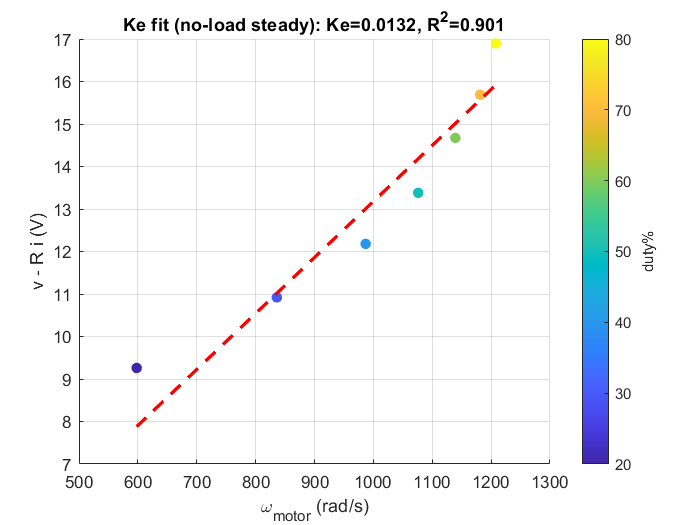
\includegraphics[width=\textwidth]{Figures/report/mech_motor_id1.png}
  \caption{Coast-down and no-load identification (Scenario 1 \& 2).}
\end{subfigure}
\hfill
\begin{subfigure}[b]{0.48\textwidth}
  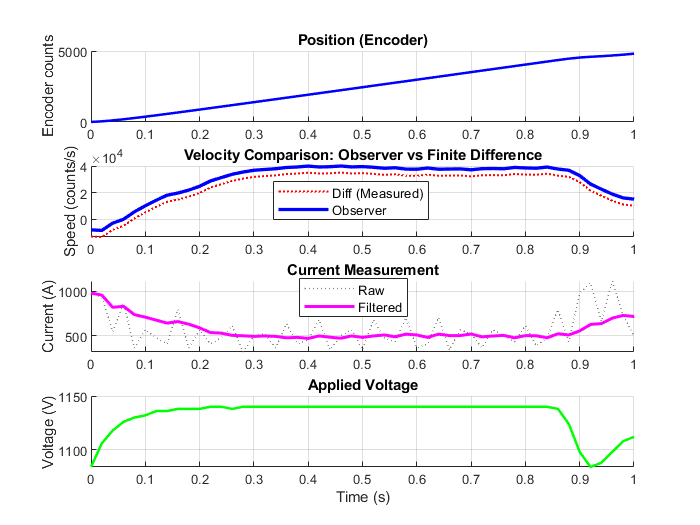
\includegraphics[width=\textwidth]{Figures/report/mech_motor_id2.png}
  \caption{Step and low-duty electrical regression (Scenario 3 \& 4).}
\end{subfigure}
\caption{Motor identification: coast-down decay and no-load electrical regression.}
\label{fig:mech_motor_identification_placeholder}
\end{figure}

\subsubsection{Isaac Sim Validation}\label{sec:isaac}
The URDF was imported into Isaac Sim as a physics articulation carrying the CAD inertials and SDF collisions. Joint limits, the passive-wrist coupling, and stable SDF contacts were verified. Static torques reproduced $G(\mathbf{q})$ \eqref{eq:G}, and acceleration responses matched $M(\mathbf{q})$ \eqref{eq:M}. The kinematics matched \texttt{works/} to numerical precision: FK to $5.6\times10^{-17}\,\mathrm{m}$, analytic IK to a worst-case $\mechSI{0.21}{mm}$ over $\sim$4500 targets with no failures, and the firmware port to $\sim1.7\times10^{-13}\,\mathrm{mm}$. These residuals confirm that the real arm, the planning model, and the twin agree to within numerical precision.

\begin{figure}[!htbp]
\centering
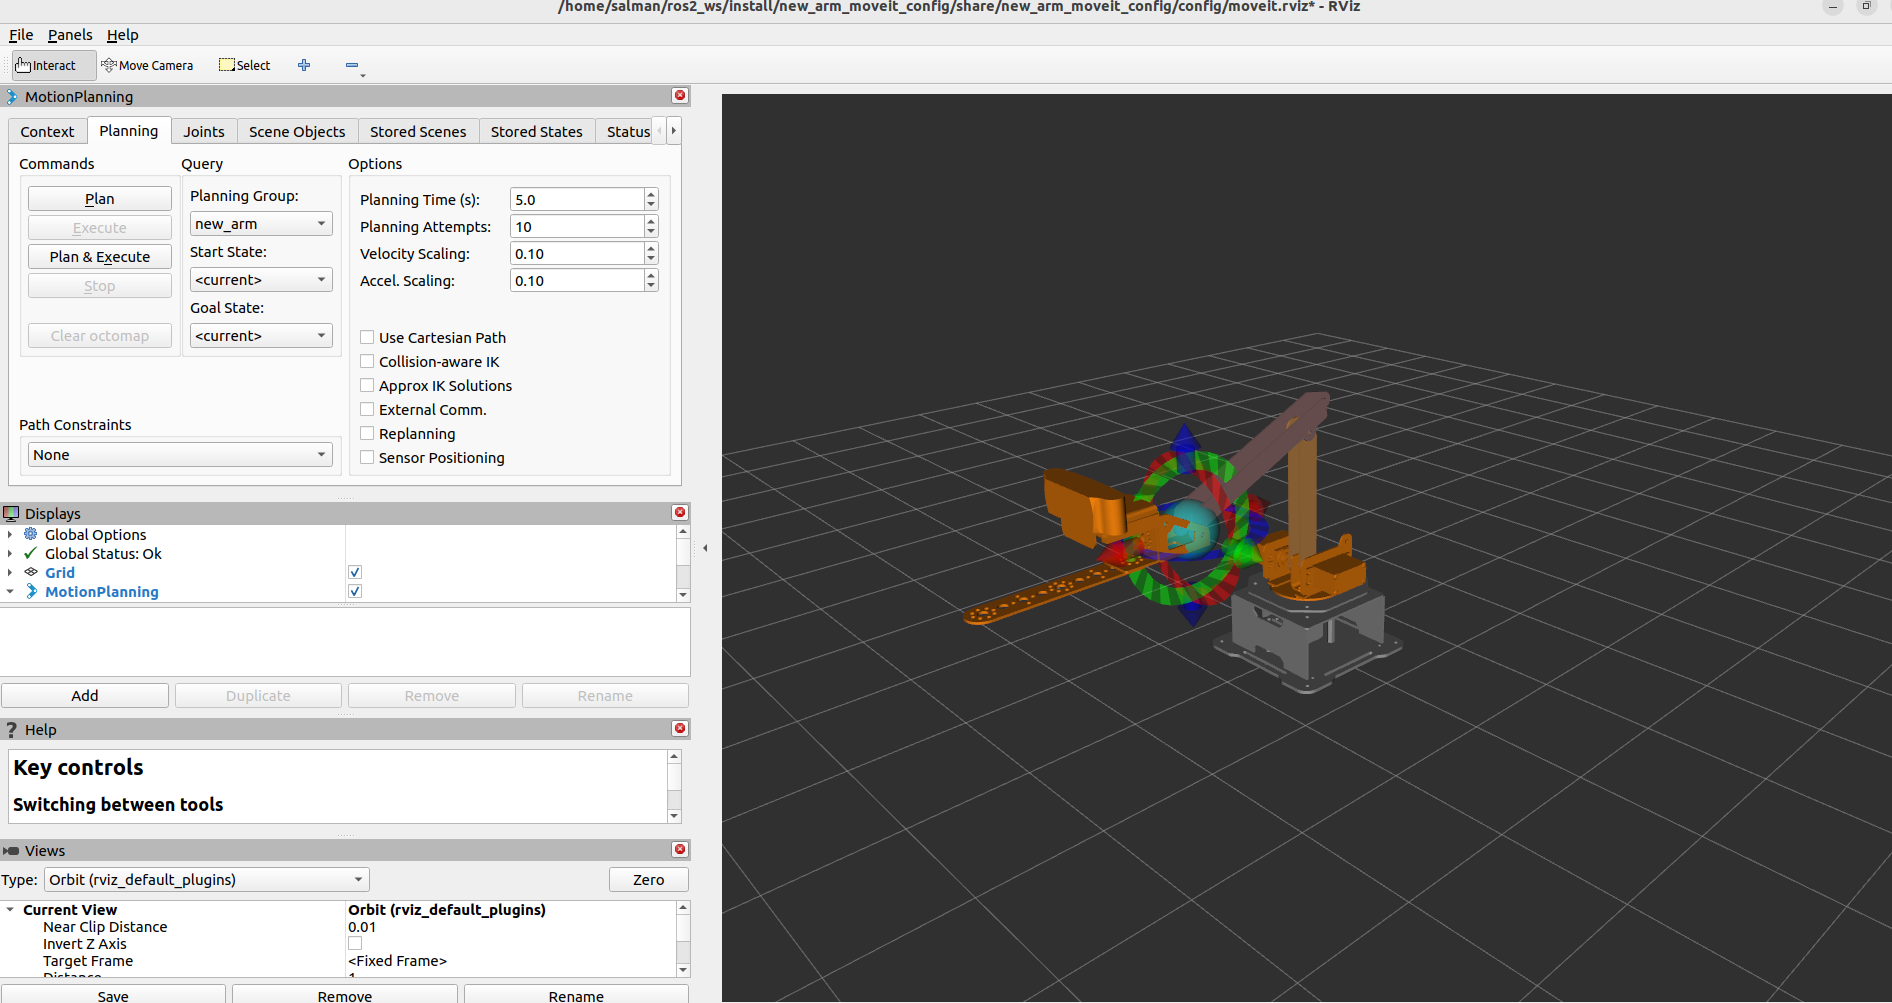
\includegraphics[width=0.88\textwidth]{Figures/report/mech_digital_twin.png}
\caption{Validation of the digital twin against the hardware and the reference kinematics.}
\label{fig:mech_digital_twin_validation_placeholder}
\end{figure}

